\newpage
\begin{abox}
	Practise Set-1
\end{abox}
\begin{enumerate}
	
	\item The Fourier transform of the derivative of the Dirac $\delta-$ function, namely $\delta^{\prime}(x)$, is proportional to
	{\exyear{NET/JRF(DEC-2013)}}
	
	\begin{tasks}(4)
		\task[\textbf{A.}] 0
		\task[\textbf{B.}] 1
		\task[\textbf{C.}] $\sin k$
		\task[\textbf{D.}] $i k$
	\end{tasks}

	\begin{answer}
		\begin{align*}
		\text{Fourier transform of }\delta^{\prime}(x)\\
		H(K)=\int_{-\infty}^{\infty} \delta^{\prime}(x) e^{i k x} d x&=i k e^{(k \cdot 0)}=i k
		\end{align*}
		So the correct answer is \textbf{Option (D)}
	\end{answer}
\item  $f(x)$ for the range $[-\infty, \infty]$ is shown below {\exyear{NET/JRF(DEC-2014)}}
	\begin{figure}[H]
		\centering
		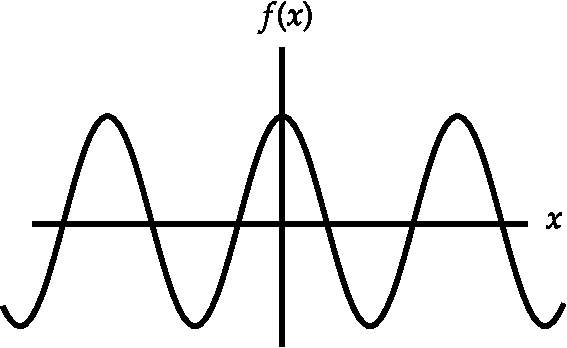
\includegraphics[height=3cm,width=5cm]{FT01}
	\end{figure}
	Which of the following graphs represents the real part of its Fourier transform?
	\begin{tasks}(2)
		\task[\textbf{A.}]
		\begin{figure}[H]
			\centering
			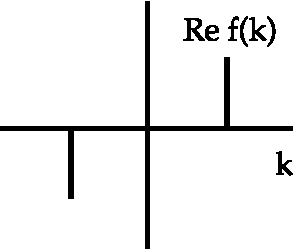
\includegraphics[height=2cm,width=2.5cm]{FT-06}
		\end{figure}
		\task[\textbf{B.}]	\begin{figure}[H]
			\centering
			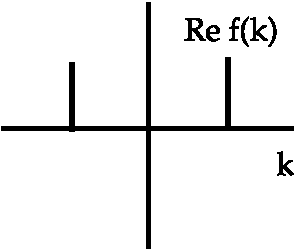
\includegraphics[height=2cm,width=2.5cm]{FT-05}
		\end{figure}
		\task[\textbf{C.}]	\begin{figure}[H]
			\centering
			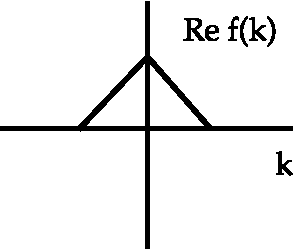
\includegraphics[height=2cm,width=2.5cm]{FT-03}
		\end{figure}
		\task[\textbf{D.}] 	\begin{figure}[H]
			\centering
			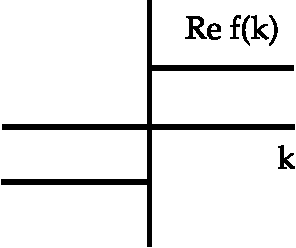
\includegraphics[height=2cm,width=2.5cm]{FT02}
		\end{figure}
	\end{tasks}
\begin{answer}
	\begin{align*}
	\text{This is cosine function}\\
	f(x)&=A \cos x \\ F(k)&=\frac{A}{2}\left[\delta\left(k-k_{0}\right)+\delta\left(k+k_{0}\right)\right]
	\end{align*}
	So the correct answer is \textbf{Option (B)}
\end{answer}
	\item The Fourier transform of $f(x)$ is $\tilde{f}(k)=\int_{-\infty}^{+\infty} d x e^{i k x} f(x)$.
	If $f(x)=\alpha \delta(x)+\beta \delta^{\prime}(x)+\gamma \delta^{\prime \prime}(x)$, where $\delta(x)$ is the Dirac delta-function (and prime denotes derivative), what is $\tilde{f}(k) ?$
	{\exyear{NET/JRF(DEC-2015)}}
	
	\begin{tasks}(2)
		\task[\textbf{A.}] $\alpha+i \beta k+i \gamma k^{2}$
		\task[\textbf{B.}] $\alpha+\beta k-\gamma k^{2}$
		\task[\textbf{C.}]  $\alpha-i \beta k-\gamma k^{2}$
		\task[\textbf{D.}] $i \alpha+\beta k-i \gamma k^{2}$
	\end{tasks}
\begin{answer}
	\begin{align*}
	\tilde{f}(k)&=\int_{-\infty}^{\infty} d x e^{i k x}\left(\alpha \delta(x)+\beta \delta^{\prime}(x)+\gamma \delta^{\prime \prime}(x)\right)\\
	\int_{-\infty}^{\infty} \alpha \delta(x) e^{i k x} d x&=\alpha\\
	\int_{-\infty}^{\infty} \beta \delta^{\prime}(x) e^{i k x} d x&=\beta\left[\left.e^{i k x} \delta(x)\right|_{-\infty} ^{\infty}-\int_{-\infty}^{\infty} i k e^{i k x} \delta(x) d x\right]=-i \beta k\\
	\int_{-\infty}^{\infty} \gamma \delta^{\prime \prime}(x) e^{i k x} d x&=-\gamma k^{2}
	\end{align*}
	So the correct answer is \textbf{Option (C)}
\end{answer}
	\item What is the Fourier transform $\int d x e^{i l x} f(x)$ of
	$$
	f(x)=\delta(x)+\sum_{n=1}^{\infty} \frac{d^{n}}{d x^{n}} \delta(x)
	$$
	where $\delta(x)$ is the Dirac delta-function?
	{\exyear{NET/JRF(JUNE-2016)}}
	
	\begin{tasks}(4)
		\task[\textbf{A.}]  $\frac{1}{1-i k}$
		\task[\textbf{B.}] $\frac{1}{1+i k}$
		\task[\textbf{C.}] $\frac{1}{k+i}$
		\task[\textbf{D.}] $\frac{1}{k-i}$
	\end{tasks}
\begin{answer}
	\begin{align*}
	f(x)&=\delta(x)+\sum_{n=1}^{\infty} \frac{d^{n}}{d x^{n}} \delta(x)\\&=\sum_{n=0}^{\infty} \frac{d^{n}}{d x^{n}} \delta(x)=\sum_{n=0}^{\infty} \delta^{(n)}(x)\\
	\because F[\delta(x)]&=1 \Rightarrow F\left[\delta^{(n)}(x)\right]\\&=(-i k)^{n} F[\delta(x)]=(-i k)^{n}\\
	\because f(x)&=\sum_{n=0}^{\infty} \delta^{(n)}(x)\\
	\Rightarrow F[f(x)]&=\sum_{n=0}^{\infty}(-i k)^{n}=1-i k+(i k)^{2}-(i k)^{3}+\ldots .\\&=\frac{1}{1-(-i k)}=\frac{1}{1+i k}
	\end{align*}
	So the correct answer is \textbf{Option (B)}
\end{answer}
	\item The Fourier transform $\int_{-\infty}^{\infty} d x f(x) e^{i k x}$ of the function $f(x)=\frac{1}{x^{2}+2}$ is
	{\exyear{NET/JRF(DEC-2016)}}
	
	\begin{tasks}(4)
		\task[\textbf{A.}] $\sqrt{2} \pi e^{-\sqrt{2}|| \mid}$
		\task[\textbf{B.}] $\sqrt{2} \pi e^{-\sqrt{2 k}}$
		\task[\textbf{C.}] $\frac{\pi}{\sqrt{2}} e^{-\sqrt{2 k}}$
		\task[\textbf{D.}] $\frac{\pi}{\sqrt{2}} e^{-\sqrt{2}|k|}$
	\end{tasks}
	\begin{answer}
		\begin{align*}
		\text{Fourier transform of }f(x)&=\frac{1}{x^{2}+a^{2}}, \\ a>0\text{ is }\int \frac{1}{x^{2}+a^{2}} e^{i k x} d x&=\frac{\pi}{a} e^{-a|k|}\\
		\text{Hence }\int \frac{1}{x^{2}+a^{2}} e^{i k x} d x&=\frac{\pi}{\sqrt{2}} e^{-\sqrt{2}|k|}
		\end{align*}
		So the correct answer is \textbf{Option (D)}
	\end{answer}
	\item The Fourier transform $\int_{-\infty}^{\infty} d x f(x) e^{i k x}$ of the function $f(x)=e^{-|x|}$
	{\exyear{NET/JRF(JUNE-2018)}}
	
	\begin{tasks}(4)
		\task[\textbf{A.}] $-\frac{2}{1+k^{2}}$
		\task[\textbf{B.}] $-\frac{1}{2\left(1+k^{2}\right)}$
		\task[\textbf{C.}] $\frac{2}{1+k^{2}}$
		\task[\textbf{D.}] $\frac{2}{\left(2+k^{2}\right)}$
	\end{tasks}
\begin{answer}
	\begin{align*}
	\int_{-\infty}^{+\infty} d x e^{-|x|} e^{i k x}&=\int_{-\infty}^{+\infty} d x e^{-|x|} \cos k x d x\text{ odd functions in }k x\text{ vanishes}\\
	\Rightarrow 2 \int_{0}^{\infty} e^{-x} \cos k x d x&=2 \frac{e^{-x}}{1+k^{2}}[-\cos k x+k \sin k x]_{0}^{\infty}\\
	\because \int e^{a x} \cos b x d x&=\frac{e^{a x}}{a^{2}+b^{2}}[a \cos b x+b \sin b x]\\
	\Rightarrow 2 \int_{0}^{\infty} e^{-x} \cos k x d x&=2 \frac{e^{0}}{1+k^{2}}=\frac{2}{1+k^{2}}
	\end{align*}
	So the correct answer is \textbf{Option (C)}
\end{answer}
	\item The Heaviside function is defined as $H(t)=\left\{\begin{array}{ll}+1, & \text { for } t>0 \\ -1, & \text { for } t<0\end{array}\right.$ and its Fourier transform is given by $-2 i / \omega$. The Fourier transform of $\frac{1}{2}[H(t+1 / 2)-H(t-1 / 2)]$ is
	{\exyear{GATE 2015}}
	
	\begin{tasks}(4)
		\task[\textbf{A.}] $\frac{\sin \left(\frac{\omega}{2}\right)}{\frac{\omega}{2}}$
		\task[\textbf{B.}]  $\frac{\cos \left(\frac{\omega}{2}\right)}{\frac{\omega}{2}}$
		\task[\textbf{C.}] $\sin \left(\frac{\omega}{2}\right)$
		\task[\textbf{D.}]  0
	\end{tasks}
\begin{answer}
	\begin{align*}
	H(f)=\int_{-\infty}^{\infty} H(t) e^{-i 2 \pi f t} d t,\text{ for a function }&H(t), H(f)=-\frac{2 i}{\omega}\\
	\text{	For }H\left(t-t_{0}\right),\text{ Fourier Transform is }&e^{-i 2 \pi f_{0}} H(f)\\
	\text{Shifting Theorem}\\
	\text{For } \frac{1}{2}\left[H\left(t+\frac{1}{2}\right)-H\left(t-\frac{1}{2}\right)\right]&=\frac{1}{2}\left[e^{i \frac{\omega}{2}}-e^{-i \frac{\omega}{2}}\right] \frac{-2 i}{\omega}\\&=\frac{1}{2 i}\left[e^{i \frac{\omega}{2}}-e^{-i \frac{\omega}{2}}\right] \frac{-2 i}{\omega} \times i\\
	\text{The Fourier transform of }\frac{1}{2}[H(t+1 / 2)-H(t-1 / 2)]&=\frac{\sin \left(\frac{\omega}{2}\right)}{\frac{\omega}{2}}
	\end{align*}
	So the correct answer is \textbf{Option (A)}
\end{answer}
	\item The Fourier transform of the function $\frac{1}{x^{4}+3 x^{2}+2}$ up to proportionality constant is
	{\exyear{JEST 2017}}
	
	\begin{tasks}(2)
		\task[\textbf{A.}] $\sqrt{2} \exp \left(-k^{2}\right)-\exp \left(-2 k^{2}\right)$
		\task[\textbf{B.}]$\sqrt{2} \exp (-|k|)-\exp (-\sqrt{2}|k|)$
		\task[\textbf{C.}] $\sqrt{2} \exp (-\sqrt{|k|})-\exp (-\sqrt{2|k|})$
		\task[\textbf{D.}]$\sqrt{2} \exp \left(-\sqrt{2} k^{2}\right)-\exp \left(-2 k^{2}\right)$
	\end{tasks}
	\begin{answer}
		\begin{align*}
		f(x)&=\frac{1}{\left(x^{4}+3 x^{2}+2\right)}=\frac{1}{\left(x^{2}+1\right)}-\frac{1}{\left[x^{2}+(\sqrt{2})^{2}\right]}\\
		\intertext{Now, Fourier transform of f(x) is,}\\
		F(p)&=A \int_{-\infty}^{\infty} f(x) e^{-1 k x} d x\\
		&=A \int_{-\infty}^{\infty}\left[\frac{1}{\left(x^{2}+1\right)}-\frac{1}{x^{2}+(\sqrt{2})^{2}}\right] e^{-i k x} d x\\&=A\left[\int_{-\infty}^{\infty} \frac{1}{\left(x^{2}+1\right)} \times e^{-i k x} d x-\int_{-\infty}^{\infty} \frac{e^{-i k x}}{x^{2}+(\sqrt{2})^{2}} d x\right]\\
		\because \int_{-\infty}^{\infty} \frac{1}{\left(x^{2}+a^{2}\right)} e^{-i k x} d x&=\sqrt{\frac{\pi}{2}} \frac{e^{-a|k|}}{a}\\
		F(k)&=A\left[\sqrt{\frac{\pi}{2}} \frac{e^{-|k|}}{1}-\sqrt{\frac{\pi}{2}} \frac{e^{-\sqrt{2}|k|}}{\sqrt{2}}\right]\\&=\frac{A \sqrt{\pi}}{2}[\sqrt{2} \exp (-|k|)-\exp (-\sqrt{2}|k|)]
		\end{align*}
		Correct option is (\textbf{option(B)})
	\end{answer}
\end{enumerate}
\colorlet{ocre1}{ocre!70!}
\colorlet{ocrel}{ocre!30!}
\setlength\arrayrulewidth{1pt}
\begin{table}[H]
	\centering
	\arrayrulecolor{ocre}
	\begin{tabular}{|p{1.5cm}|p{1.5cm}||p{1.5cm}|p{1.5cm}|}
		\hline
		\multicolumn{4}{|c|}{\textbf{Answer key}}\\\hline\hline
		\rowcolor{ocrel}Q.No.&Answer&Q.No.&Answer\\\hline
		1&\textbf{D} &2&\textbf{B}\\\hline 
		3&\textbf{C} &4&\textbf{B} \\\hline
		5&\textbf{D} &6&\textbf{C} \\\hline
		7&\textbf{A}&8&\textbf{B}\\\hline
		
		
	\end{tabular}
\end{table}
\newpage
\begin{abox}
	Problem Set-2
\end{abox}
\begin{enumerate}
	\item The graph of the function $f(x)=\left\{\begin{array}{ll}1 & \text { for } 2 n \leq x \leq 2 n+1 \\ 0 & \text { for } 2 n+1 \leq x \leq 2 n+2\end{array}\right.$ where $n=(0,1,2, \ldots \ldots)$ is shown below. Its Laplace transform $\tilde{f}(s)$ is
	{	\exyear{NET/JRF(DEC-2011)}}
	
	\begin{figure}[H]
		\centering
		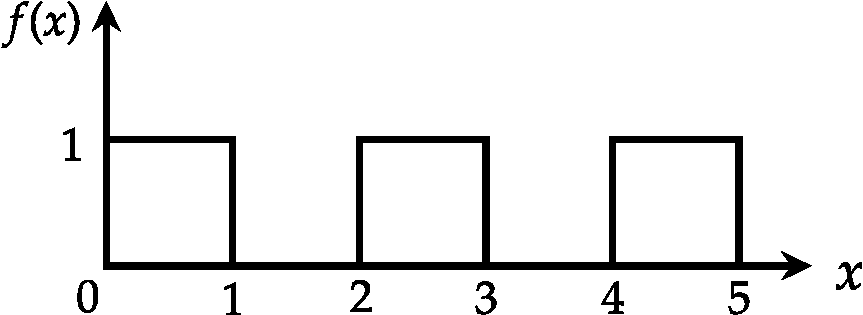
\includegraphics[height=2.7cm,width=7.5cm]{diagram-20211005(9)-crop}
	\end{figure}
	\begin{tasks}(4)
		\task[\textbf{A.}] $\frac{1+e^{-s}}{s}$
		\task[\textbf{B.}] $\frac{1-e^{-s}}{s}$
		\task[\textbf{C.}] $\frac{1}{s\left(1+e^{-s}\right)}$
		\task[\textbf{D.}]  $\frac{1}{s\left(1-e^{-s}\right)}$
	\end{tasks}
	\begin{answer}
		\begin{align*}
		L(f(x))&=\int_{0}^{\infty} e^{-s x} f(x) d x\\&=\int_{0}^{1} e^{-s x} \cdot 1 d x+\int_{1}^{2} e^{-s x} \cdot 0 d x+\int_{2}^{3} e^{-s x} \cdot 1 d x+\ldots \ldots\\
		&=\left[\frac{e^{-s x}}{-s}\right]_{0}^{1}+0+\left[\frac{e^{-s x}}{-s}\right]_{2}^{3}+\ldots \ldots\\&=\frac{1}{-s}\left[e^{-s}-1\right]+\frac{1}{-s}\left[e^{-3 s}-e^{-2 s}\right]+\ldots \ldots\\
		&=\frac{1}{-s}\left[-1+e^{-s}-e^{-2 s}+e^{-3 s}+\ldots \ldots . .\right]\\&=\frac{1}{s}\left[1-e^{-s}+e^{-2 s}-e^{-3 s}+\ldots .\right]\\
		\text{Since }S_{\infty}&=\frac{a}{1-r}\text{ where }r=-e^{-s}\text{ and }a\\&=1 \Rightarrow S_{\infty}=\frac{1}{s}\left[\frac{1}{\left(1+e^{-s}\right)}\right]
		\end{align*}
		So the correct answer is \textbf{Option(C)}
	\end{answer}
	\item The inverse Laplace transforms of $\frac{1}{s^{2}(s+1)}$ is
	{\exyear{NET/JRF(JUNE-2013)}}
	
	\begin{tasks}(4)
		\task[\textbf{A.}] $\frac{1}{2} t^{2} e^{-t}$
		\task[\textbf{B.}] $\frac{1}{2} t^{2}+1-e^{-t}$
		\task[\textbf{C.}] $t-1+e^{-t}$
		\task[\textbf{D.}] $\frac{1}{2} t^{2}\left(1-e^{-t}\right)$
	\end{tasks}
	\begin{answer}
		\begin{align*}
		f(s)&=\frac{1}{s+1} \Rightarrow f(t)=e^{-t} \Rightarrow L^{-1}\left[\frac{1}{s(s+1)}\right]\\&=\int_{0}^{t} e^{-t} d t=\left(-e^{-t}\right)_{0}^{t}=\left(-e^{-t}+1\right)\\
		\Rightarrow L^{-1}\left[\frac{1}{s^{2}(s+1)}\right]&=\int_{0}^{t}\left(-e^{-t}+1\right) d t\\&=\left(e^{-t}+t\right)_{0}^{t}=e^{-t}+t-1
		\end{align*}
		So the correct answer is \textbf{Option (C)}
	\end{answer}
	\item The Laplace transform of
	$$
	f(t)=\left\{\begin{array}{cc}
	\frac{t}{T}, & 0<t<T \\
	1 & t>T
	\end{array}\right.
	$$
	is
	{\exyear{NET/JRF(DEC-2016)}}
	
	\begin{tasks}(4)
		\task[\textbf{A.}] $\frac{-\left(1-e^{-s T}\right)}{s^{2} T}$
		\task[\textbf{B.}] $\frac{\left(1-e^{-s T}\right)}{s^{2} T}$
		\task[\textbf{C.}] $\frac{\left(1+e^{-s T}\right)}{s^{2} T}$
		\task[\textbf{D.}] $\frac{\left(1-e^{s T}\right)}{s^{2} T}$
	\end{tasks}
	\begin{answer}
		\begin{align*}
		\intertext{we can write}
		f(t)&=\left[u_{0}(t)-u_{T}(t)\right] \frac{t}{T}+u_{T}(t)\\&=\left[1-u_{T}(t)\right] \frac{t}{T}+u_{T}(t)=\frac{t}{T}-u_{T}(t) \frac{t}{T}+u_{T}(t)
		\intertext{Hence the transform of $f(t)$ is}
		L\{f(t)\}&=L\left\{\frac{t}{T}\right\}-L\left\{u_{T}(t)\left[\frac{(t-T)+T}{T}\right]\right\}+L\left\{u_{T}(t)\right\}\\
		&=\frac{1}{s^{2} T}-\frac{e^{-s T}}{T}\left(\frac{1}{s^{2}}+\frac{T}{s}\right)+\frac{e^{-s T}}{s}\\&=\frac{1-e^{-s T}}{s^{2} T}
		\end{align*}
		So the correct answer is \textbf{Option (B)}
	\end{answer}
	\item Consider the differential equation $\frac{d y}{d t}+a y=e^{-b t}$ with the initial condition $y(0)=0$. Then the Laplace transform $Y(s)$ of the solution $y(t)$ is
	{\exyear{NET/JRF(DEC-2017)}}
	
	\begin{tasks}(4)
		\task[\textbf{A.}] $\frac{1}{(s+a)(s+b)}$
		\task[\textbf{B.}] $\frac{1}{b(s+a)}$
		\task[\textbf{C.}] $\frac{1}{a(s+b)}$
		\task[\textbf{D.}] $\frac{e^{-a}-e^{-b}}{b-a}$
	\end{tasks}
	\begin{answer}
		\begin{align*}
		\text{Given }\frac{d y}{d t}+a y&=e^{-b t}
		\intertext{Taking Laplace transform of both sides}
		\text{	We obtain}\\
		L\left\{\frac{d y}{d t}\right\}+a L\{y(t)\}&=L\left\{e^{-b t}\right\} \Rightarrow s Y(s)-y(0)+a Y(s)=\frac{1}{s+b}\\
		\text{Since, }	y(0)&=0,\text{ we obtain}\\
		(s+a) Y(s)&=\frac{1}{s+b} \\ Y(s)&=\frac{1}{(s+a)(s+b)}
		\end{align*}
		So the correct answer is \textbf{Option (A)}
	\end{answer}
	\item If $f(x)=\left\{\begin{array}{ll}0 & \text { for } x<3, \\ x-3 & \text { for } x \geq 3\end{array}\right.$ then the Laplace transform of $f(x)$ is
	{\exyear{GATE 2010}}
	
	\begin{tasks}(4)
		\task[\textbf{A.}] $s^{-2} e^{3 s}$
		\task[\textbf{B.}] $s^{2} e^{3 s}$
		\task[\textbf{C.}] $s^{-2}$
		\task[\textbf{D.}] $s^{-2} e^{-3 s}$
	\end{tasks}
	\begin{answer}
		\begin{align*}
		L\{f(x)\}&=\int_{0}^{\infty} e^{-s x} f(x) d x\\&=\int_{0}^{3} e^{-s x} f(x) d x+\int_{3}^{\infty} e^{-s x} f(x) d x\\&=\int_{3}^{\infty}(x-3) e^{-s x} d x\\
		L\{f(x)\}&=\left.(x-3) \frac{e^{-s x}}{-s}\right|_{3} ^{\infty}-\int_{3}^{\infty} 1 \cdot\left(\frac{e^{-s x}}{-s}\right) d x\\&=0+\frac{1}{s} \int_{3}^{\infty} e^{-s x} d x\\&=\frac{1}{s}\left[\frac{e^{-s x}}{-s}\right]_{3}^{\infty}\\&=s^{-2} e^{-3 s}
		\end{align*}
		So the correct answer is \textbf{Option (D)}
	\end{answer}
	\item The Laplace transform of $\frac{(\sin (a t)-a t \cos (a t))}{\left(2 a^{3}\right)}$ is 
	{\exyear{JEST 2018}}
	
	\begin{tasks}(4)
		\task[\textbf{A.}] $\frac{2 a s}{\left(s^{2}+a^{2}\right)^{2}}$
		\task[\textbf{B.}]$\frac{s^{2}-a^{2}}{\left(s^{2}+a^{2}\right)^{2}}$
		\task[\textbf{C.}]$\frac{1}{(s+a)^{2}}$
		\task[\textbf{D.}]$\frac{1}{\left(s^{2}+a^{2}\right)^{2}}$
	\end{tasks}
\begin{answer}
	\begin{align*}
		L{f(t)}&=L\left\{\frac{1}{2 a^{3}}(\sin a t-a t \cos a t)\right\} \\
		&=\frac{1}{2 a^{3}}(L\left\lbrace {\sin a t}\right\rbrace -a L\left\lbrace  {t \cos a t}\right\rbrace )\\
		&=\frac{1}{2 a^{3}}\left(\frac{a}{s^{2}+a^{2}}-a\left(-\frac{d}{d s} \frac{s}{s^{2}+a^{2}}\right)\right)\\
		&=\frac{1}{2 a^{2}}\left(\frac{1}{s^{2}+a^{2}}+\left( \frac{a^{2}-s^{2}}{s^{2}+a^{2}}\right)\right)\\
		&=\frac{1}{2 a^{2}}\left(\frac{s^{2}+a^{2}}{(s^{2}+a^{2})^{2}}+\left( \frac{a^{2}-s^{2}}{s^{2}+a^{2}}\right)\right)\\
		&=\frac{1}{2 a^{2}}\left(\frac{2a^{2}}{(s^{2}+a^{2})^{2}}\right) \\
		&=\frac{1}{(s^{2}+a^{2})^{2}}
		\end{align*}
		So the correct answer is \textbf{Option(D)}
\end{answer}
\item 	 The Laplace transformation of $e^{-2 t} \sin 4 t$ is
{\exyear{JEST 2014}}

\begin{tasks}(4)
\task[\textbf{A.}] $\frac{4}{s^{2}+4 s+25}$
\task[\textbf{B.}]$\frac{4}{s^{2}+4 s+20}$
\task[\textbf{C.}]$\frac{4 s}{s^{2}+4 s+20}$
\task[\textbf{D.}]$\frac{4 s}{2 s^{2}+4 s+20}$
\end{tasks}
\begin{answer}
\begin{align*}
\because L\left[e^{-a t} \sin b t\right]&=\frac{b}{(s+a)^{2}+b^{2}}\\
\Rightarrow L\left[e^{-2 t} \sin 4 t\right]&=\frac{4}{(s+2)^{2}+4^{2}}\\&=\frac{4}{s^{2}+4 s+20}
\end{align*}
Correct option is (\textbf{Option C})
\end{answer}
\end{enumerate}
\colorlet{ocre1}{ocre!70!}
\colorlet{ocrel}{ocre!30!}
\setlength\arrayrulewidth{1pt}
\begin{table}[H]
	\centering
	\arrayrulecolor{ocre}
	\begin{tabular}{|p{1.5cm}|p{1.5cm}||p{1.5cm}|p{1.5cm}|}
		\hline
		\multicolumn{4}{|c|}{\textbf{Answer key}}\\\hline\hline
		\rowcolor{ocrel}Q.No.&Answer&Q.No.&Answer\\\hline
		1&\textbf{C} &2&\textbf{C}\\\hline 
		3&\textbf{B} &4&\textbf{A} \\\hline
		5&\textbf{D} &6 &\textbf{D} \\\hline
		7&\textbf{C} & & \\\hline
		
	\end{tabular}
\end{table}